\chapter{Conception}
This chapter describes the concept and design of the application based on the previously analyzed requirements. This chapter outlines the application's structure, functionalities, technologies, and patterns used to fulfill the listed requirements.

\section{System Architecture}
In this section, an architecture diagram is displayed to have a better understanding of the system architecture as well as its components.
\begin{figure}[H]
    \centering
    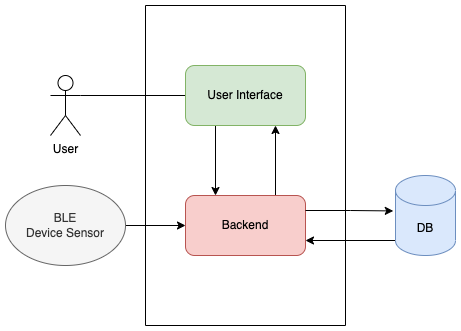
\includegraphics[width=1\textwidth]{diagrams/system-diagram.drawio.png}
    \caption{System architecture diagram}
    \label{fig:sys_diagram}
\end{figure}
\autoref{fig:sys_diagram} illustrates the components of the systems and the interaction between the components. Within the system, there are two components: the user interface and the backend which connects to a local database to store and manage data.
In addition, the device sensor is connected to the backend via bluetooth low energy and transmit the user's heart rate.

\section{Software Architecture}
Software Architecture section, show some diagrams

\section{Technologies}
Tech section
\subsection{User Interface}
talk about what tech is used for the ui
\subsection{Backend Infrastructure}
talk about what tech is used for the backend
\subsection{Database}
talk about what tech is used for the db


\section{Software Design}
the model-view-viewmodel follows the seperation of concerns principles blablabla
The MVVM pattern promotes loose coupling and separation of concerns, making the application more maintainable and testable. The View and ViewModel are often connected using data binding techniques, allowing automatic synchronization of data between the two.
By following MVVM, developers can achieve a clear separation of responsibilities, allowing for easier development, testing, and maintenance of the application.
\subsection{Model}
\subsection{View}
\subsection{ViewModel}

\section{Features}
